\chapter{Results}

This chapter reports empirical outcomes of supervised chain-of-thought distillation (SCoTD) and label-only finetuning on GSM8K. All metrics use strict numeric exact-match evaluation under greedy decoding. No self-consistency sampling or answer normalization was applied.

\section{Evaluation setup recap}
\begin{itemize}
    \item Base model: \texttt{Qwen/Qwen2.5-3B}, no finetuning.
    \item Students: LoRA adapters trained on cleaned teacher data (SCoTD: rationale+answer, Label-only: final answer line only).
    \item Teacher: \texttt{deepseek/deepseek-r1-distill-qwen-32b} via API.
    \item Decoding: greedy (\texttt{do\_sample=false}) for all benchmarks.
    \item Metric: accuracy = correct numeric parses / total questions (1{,}319 GSM8K test problems).
    \item Parsing: requires a line starting \texttt{Final Answer: } followed by a single numeric token; any deviation counts as incorrect.
\end{itemize}

\section{Headline accuracies}
\begin{itemize}
    \item Teacher (API): 93.61\%.
    \item Student SCoTD (best checkpoint): 78.54\%.
    \item Base (CoT prompting, no finetune): 70.51\%.
    \item Student label-only (best checkpoint): 15.01\%.
    \item Base (label-only prompting): 10.99\%.
\end{itemize}
Thus SCoTD yields a +8.03 percentage-point gain over the base CoT baseline, while label-only supervision gives a +4.02 point gain over the label-only baseline under strict formatting.

\section{Checkpoint dynamics}
\subsection{SCoTD}
Model saved every 200 training steps. Best accuracy observed at step 1{,}400 (78.54\%). Checkpoints after this point exhibit slight stagnation (no further gains) despite continued training loss decrease, indicating diminishing returns and potential mild overfitting to rationale style rather than numeric robustness.

\subsection{Label-only}
Saved every 50 steps; best accuracy at step 200 (15.01\%). Subsequent checkpoints degrade or plateau, correlating with rising validation loss after early minimum (Figure: label-only eval loss curve). Early stopping at the first validation-loss inflection would preserve best generalization.

\section{Training behavior}
\subsection{Label-only mode (answer line only)}
\begin{figure}[!h]
    \centering
    \begin{subfigure}[b]{0.49\linewidth}
        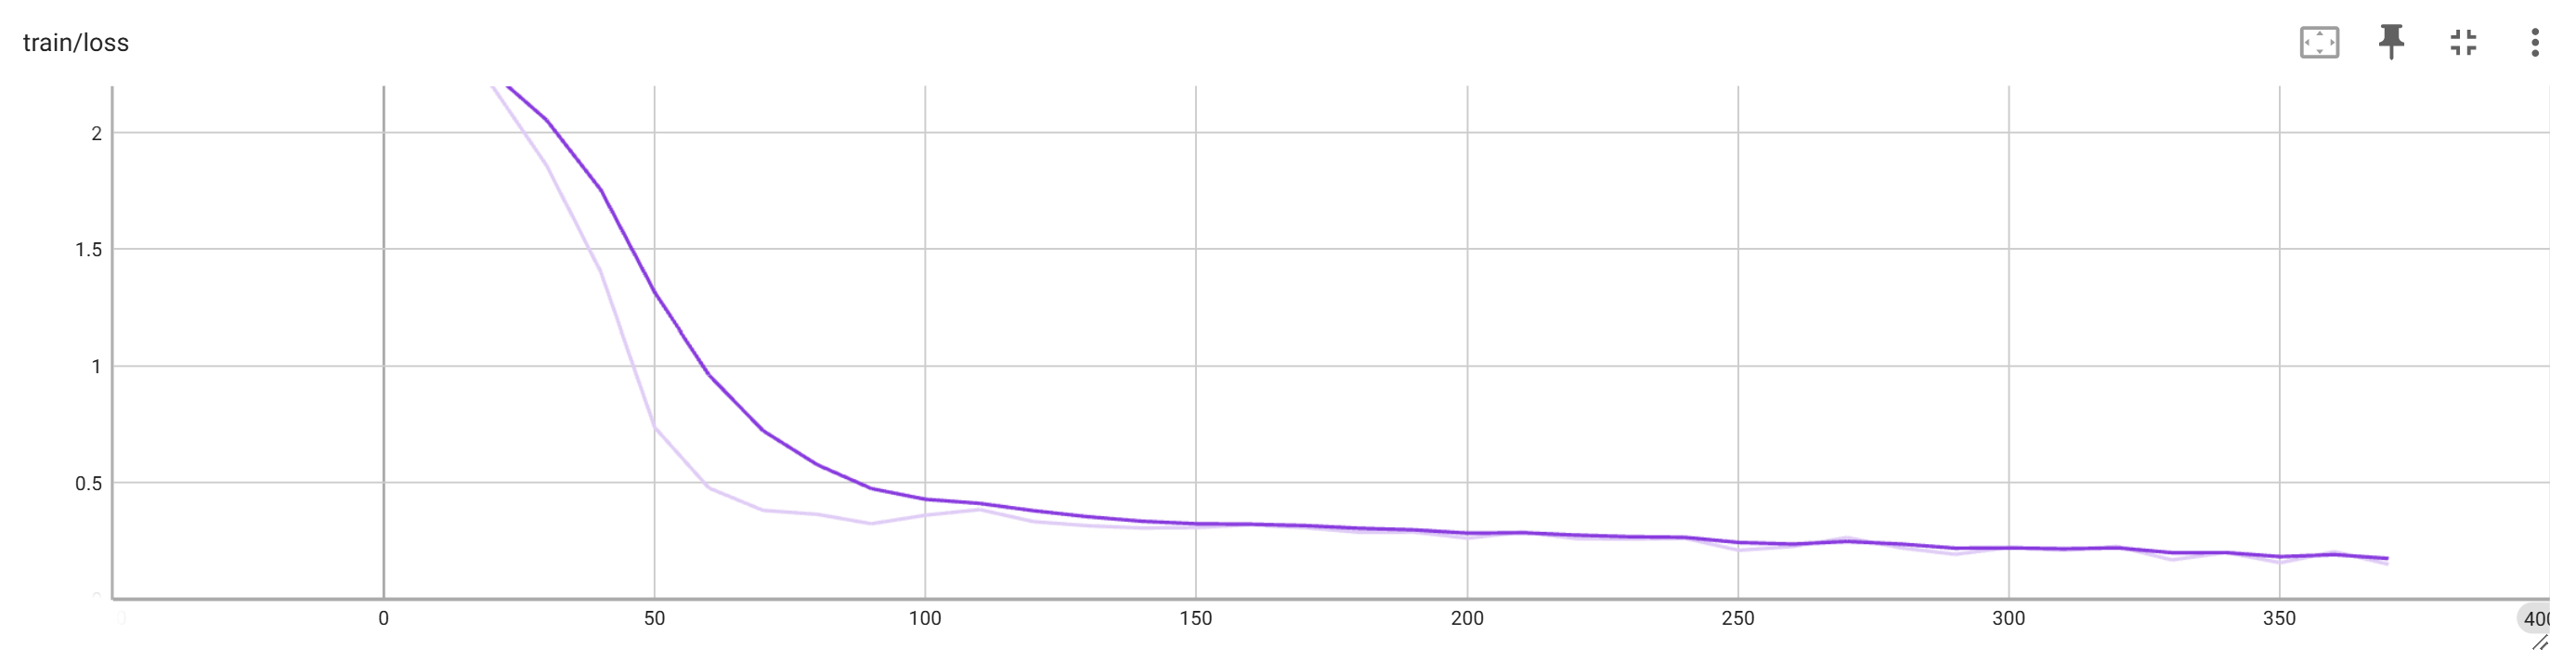
\includegraphics[width=\linewidth]{img/label_only_train_loss.png}
        \caption{Train loss}
    \end{subfigure}
    \begin{subfigure}[b]{0.49\linewidth}
        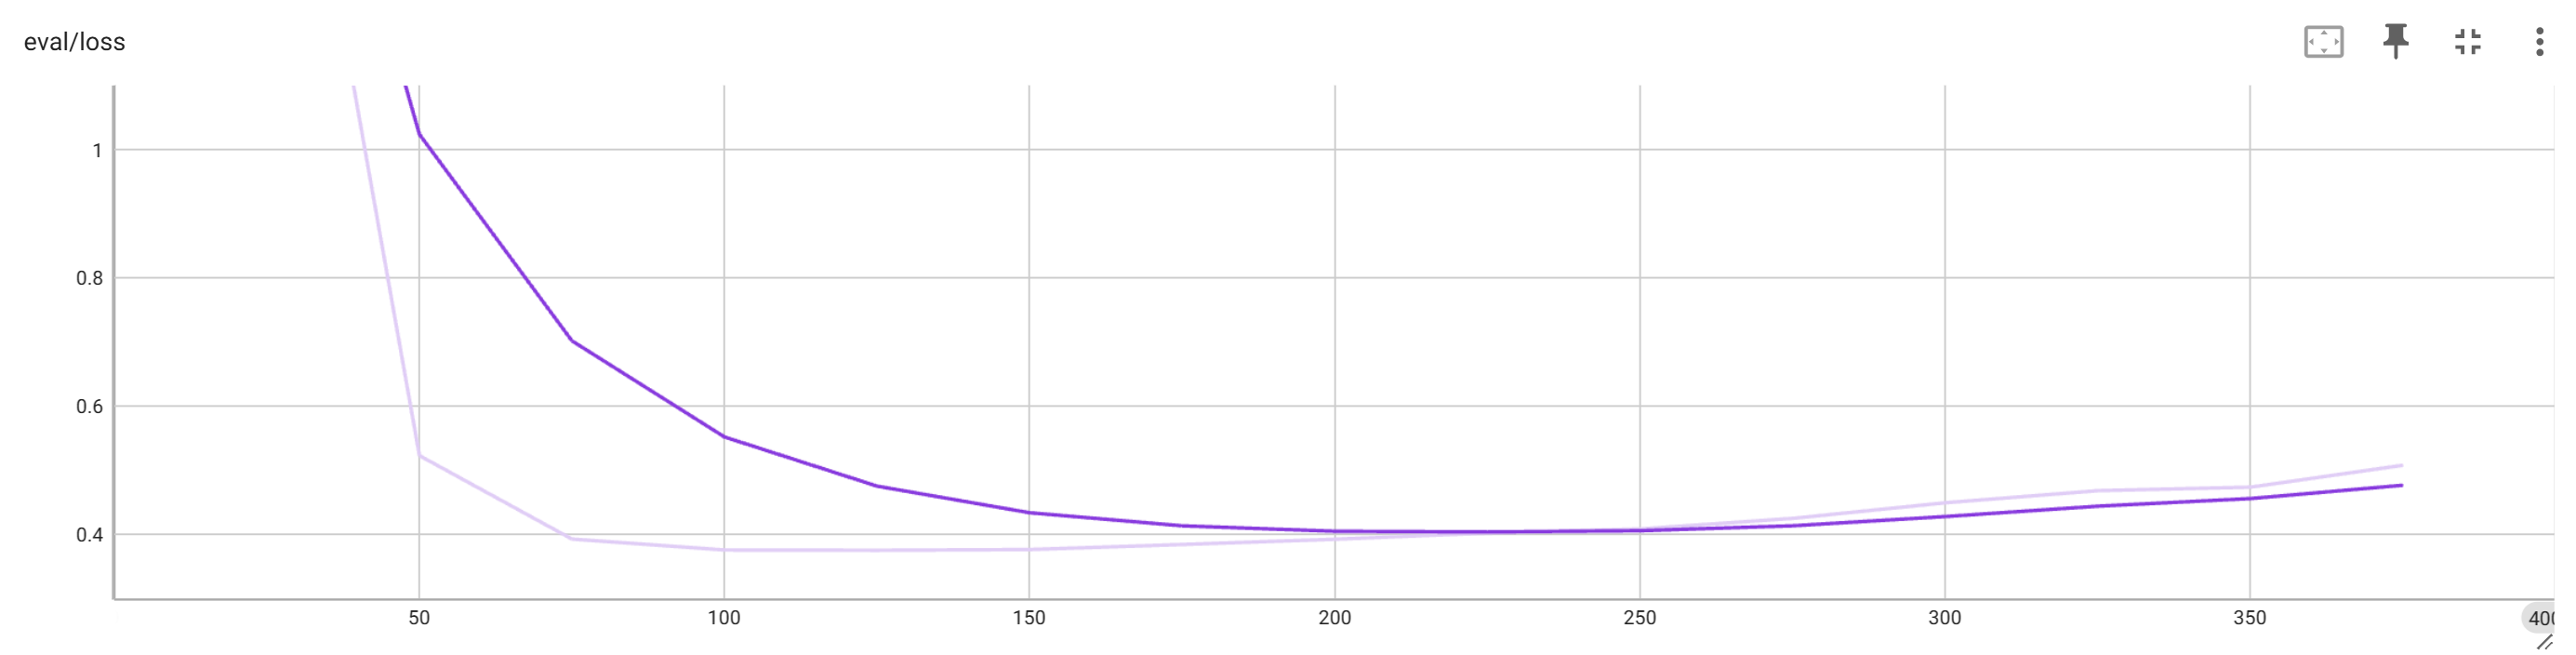
\includegraphics[width=\linewidth]{img/label_only_eval_loss.png}
        \caption{Eval loss}
    \end{subfigure}
    \caption{Label-only losses: rapid early train loss compression; eval loss reaches minimum near 180--220 steps then rises (overfitting onset).}
    \label{fig:labelonly-losses}
\end{figure}

\begin{figure}[!h]
    \centering
    \begin{subfigure}[b]{0.49\linewidth}
        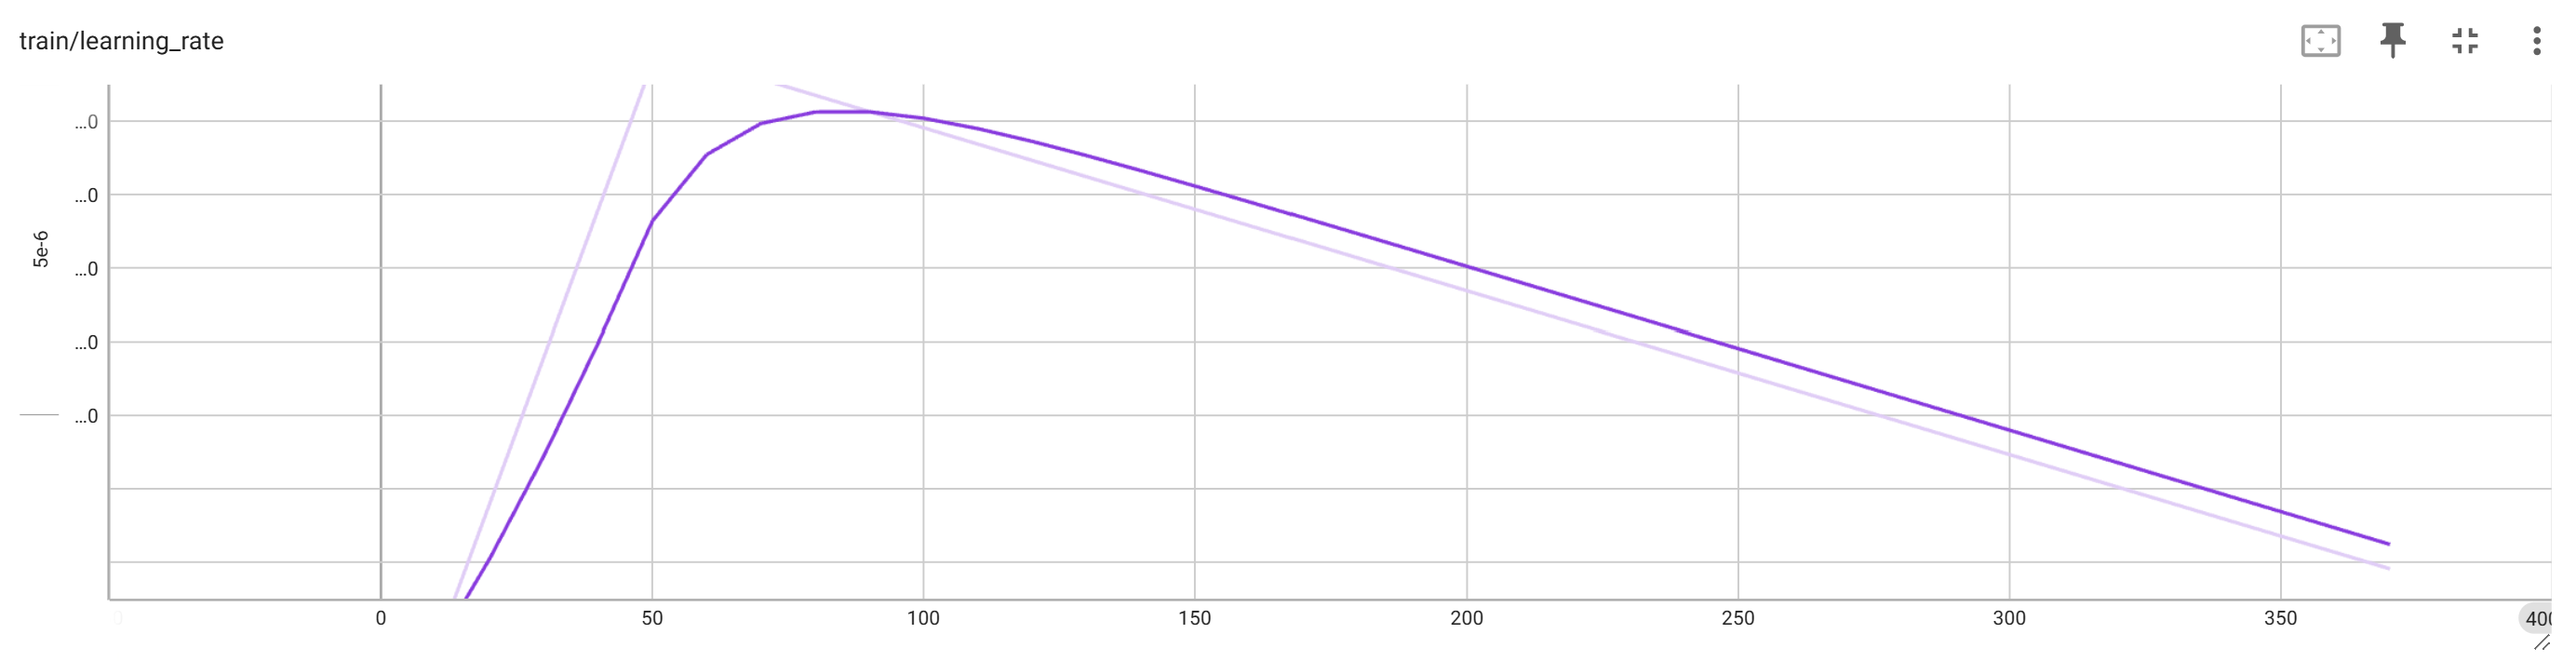
\includegraphics[width=\linewidth]{img/label_only_train_learning_rate.png}
        \caption{Learning rate}
    \end{subfigure}
    \begin{subfigure}[b]{0.49\linewidth}
        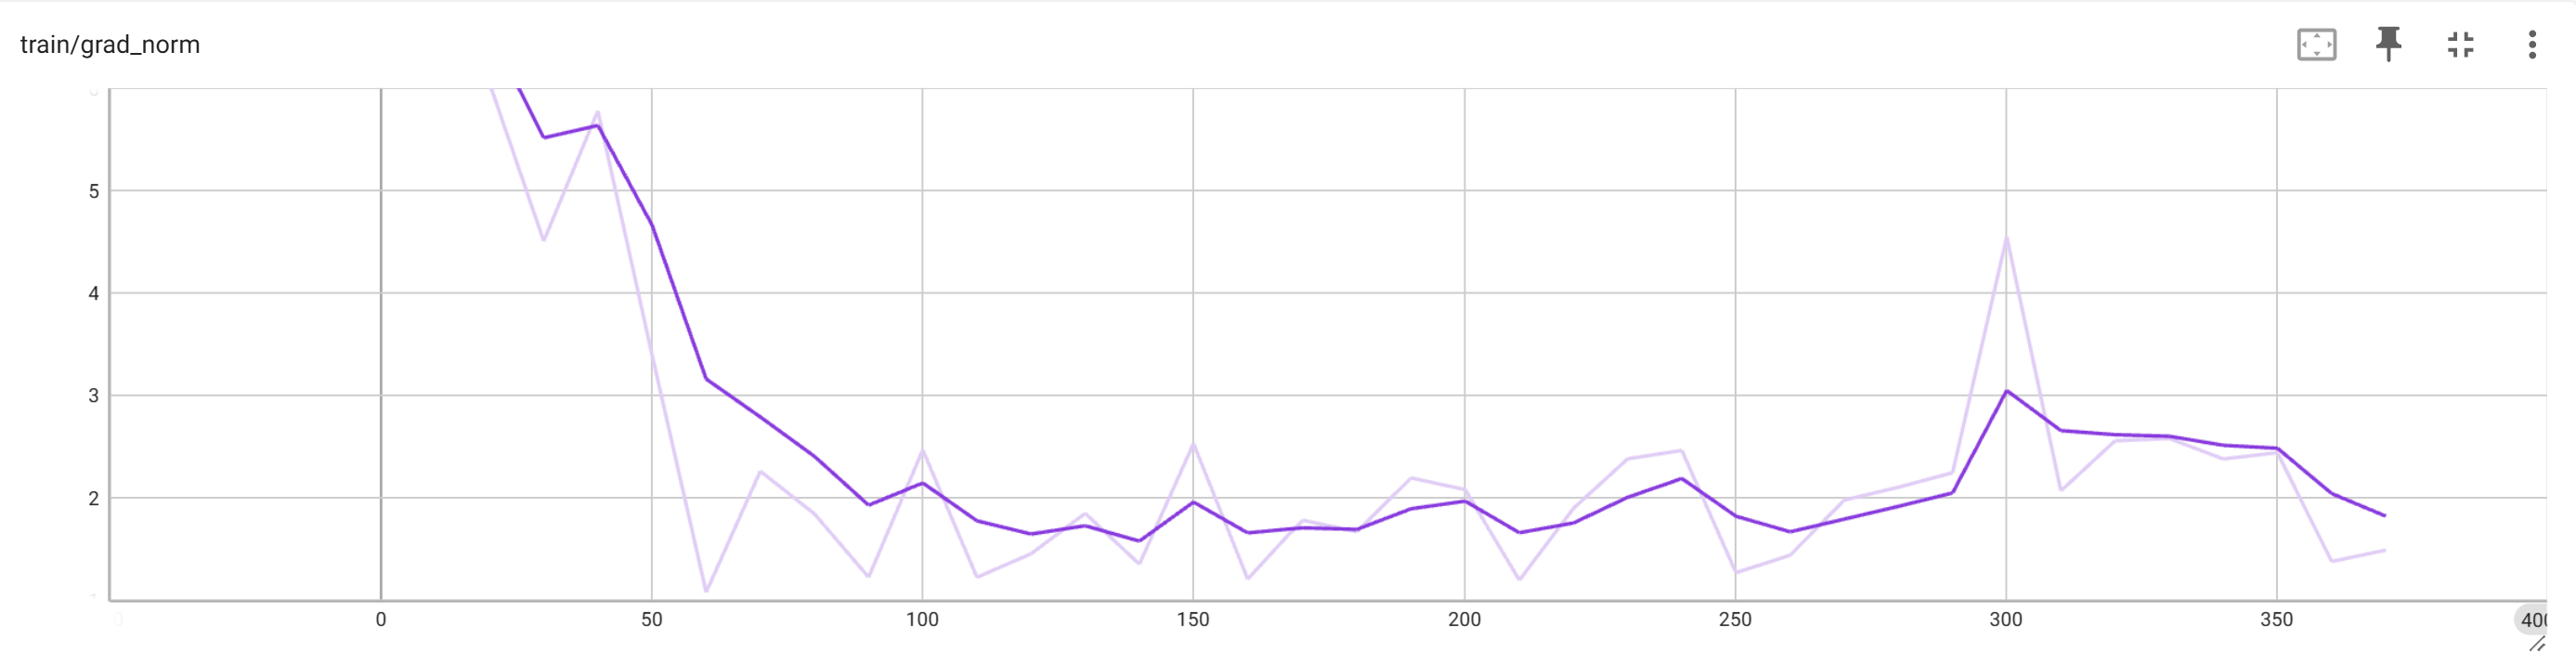
\includegraphics[width=\linewidth]{img/label_only_train_grad_norm.png}
        \caption{Grad norm}
    \end{subfigure}
    \caption{Label-only optimization dynamics: warmup then linear LR decay; early high gradient norms (>6) collapse to a stable 1.5--2.5 band.}
    \label{fig:labelonly-dynamics}
\end{figure}

Observations:
\begin{itemize}
    \item Rapid optimization: train loss drops >75\% within first \~120 steps (Figure \ref{fig:labelonly-losses}a).
    \item Generalization peak: eval loss minimum near 180--220 steps (Figure \ref{fig:labelonly-losses}b) aligns with best accuracy (15.01\%); subsequent rise indicates overfitting on formatting/token patterns.
    \item Gradient norm collapse: large initial adaptation (Figure \ref{fig:labelonly-dynamics}b) precedes eval loss floor; post-collapse stability reflects limited sequence length.
\end{itemize}

\subsection{SCoTD mode (rationale + answer)}
\begin{figure}[!h]
    \centering
    \begin{subfigure}[b]{0.49\linewidth}
        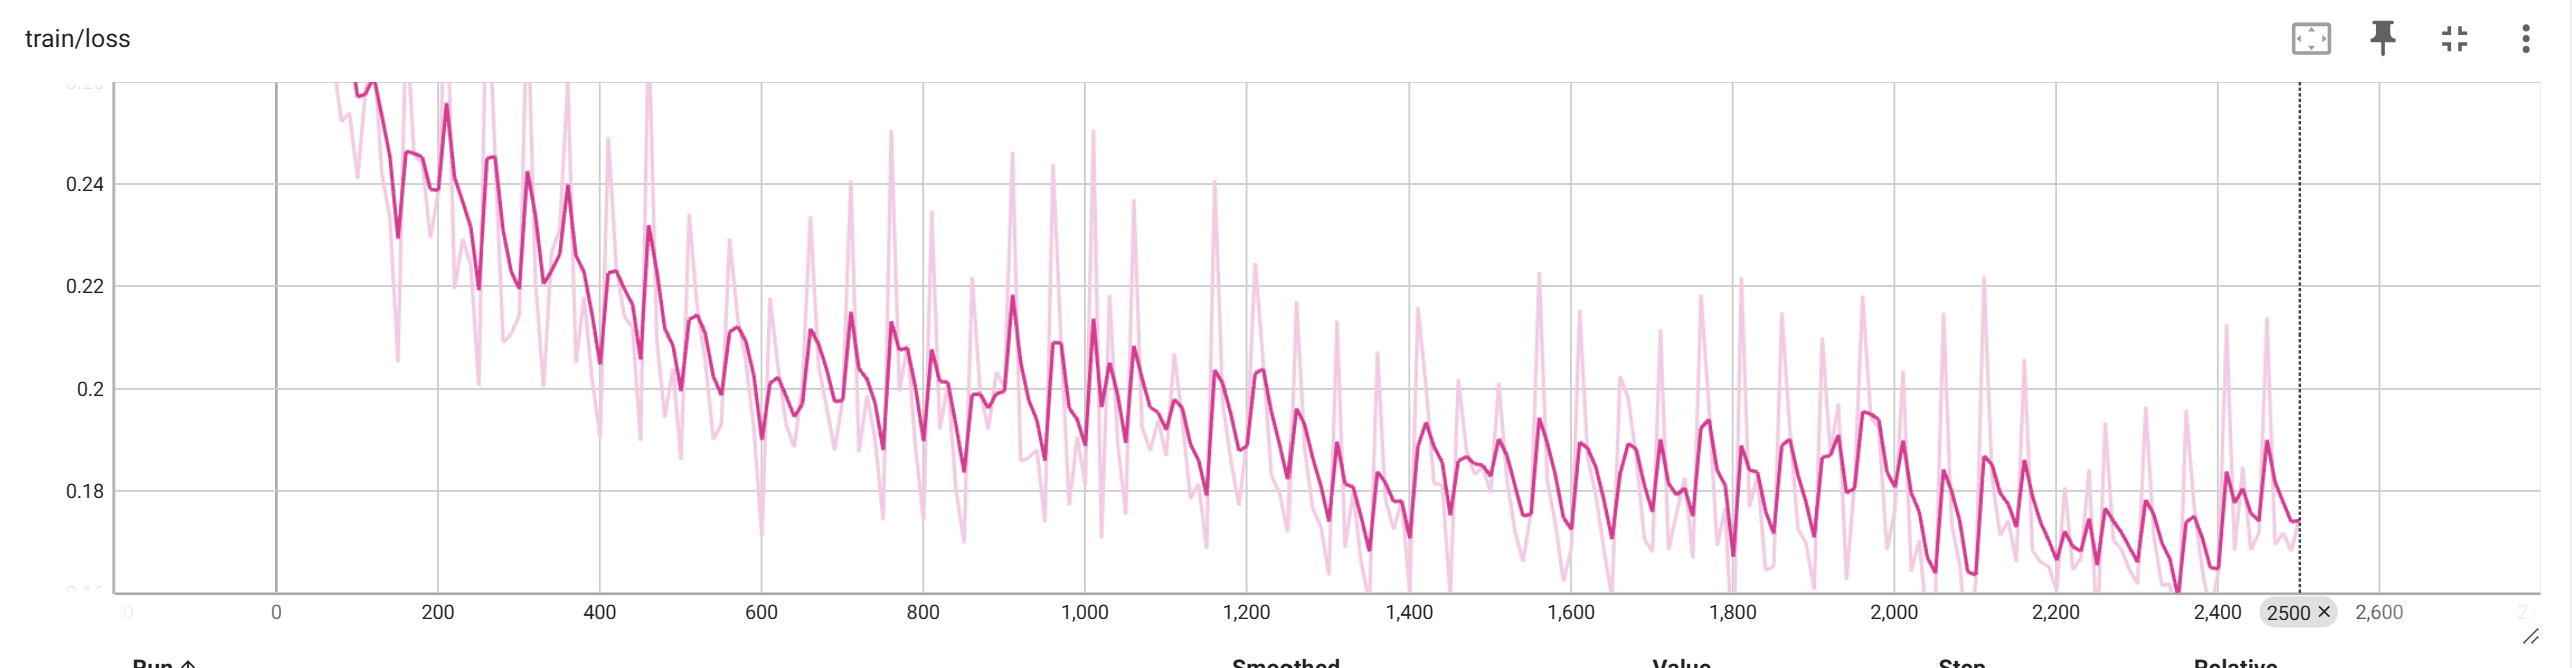
\includegraphics[width=\linewidth]{img/sctod_train_loss.png}
        \caption{Train loss}
    \end{subfigure}
    \begin{subfigure}[b]{0.49\linewidth}
        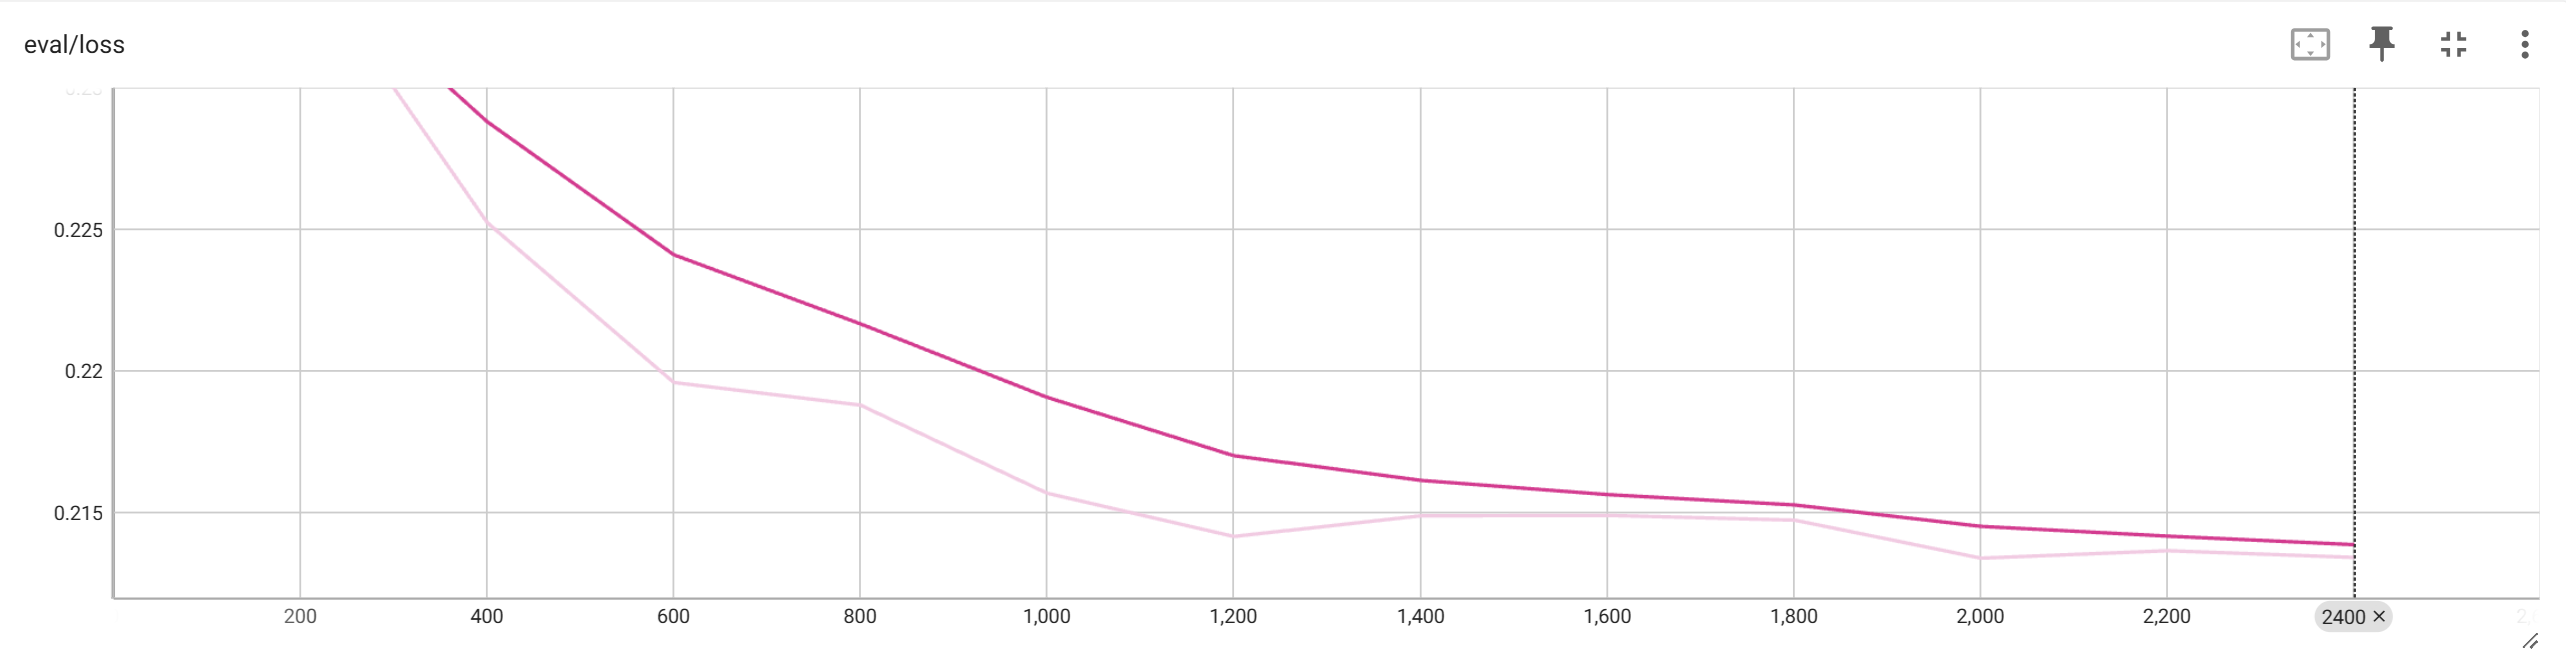
\includegraphics[width=\linewidth]{img/sctod_eval_loss.png}
        \caption{Eval loss}
    \end{subfigure}
    \caption{SCoTD losses: steady train loss descent; eval loss monotonically declines without early reversal.}
    \label{fig:sctod-losses}
\end{figure}

\begin{figure}[!h]
    \centering
    \begin{subfigure}[b]{0.49\linewidth}
        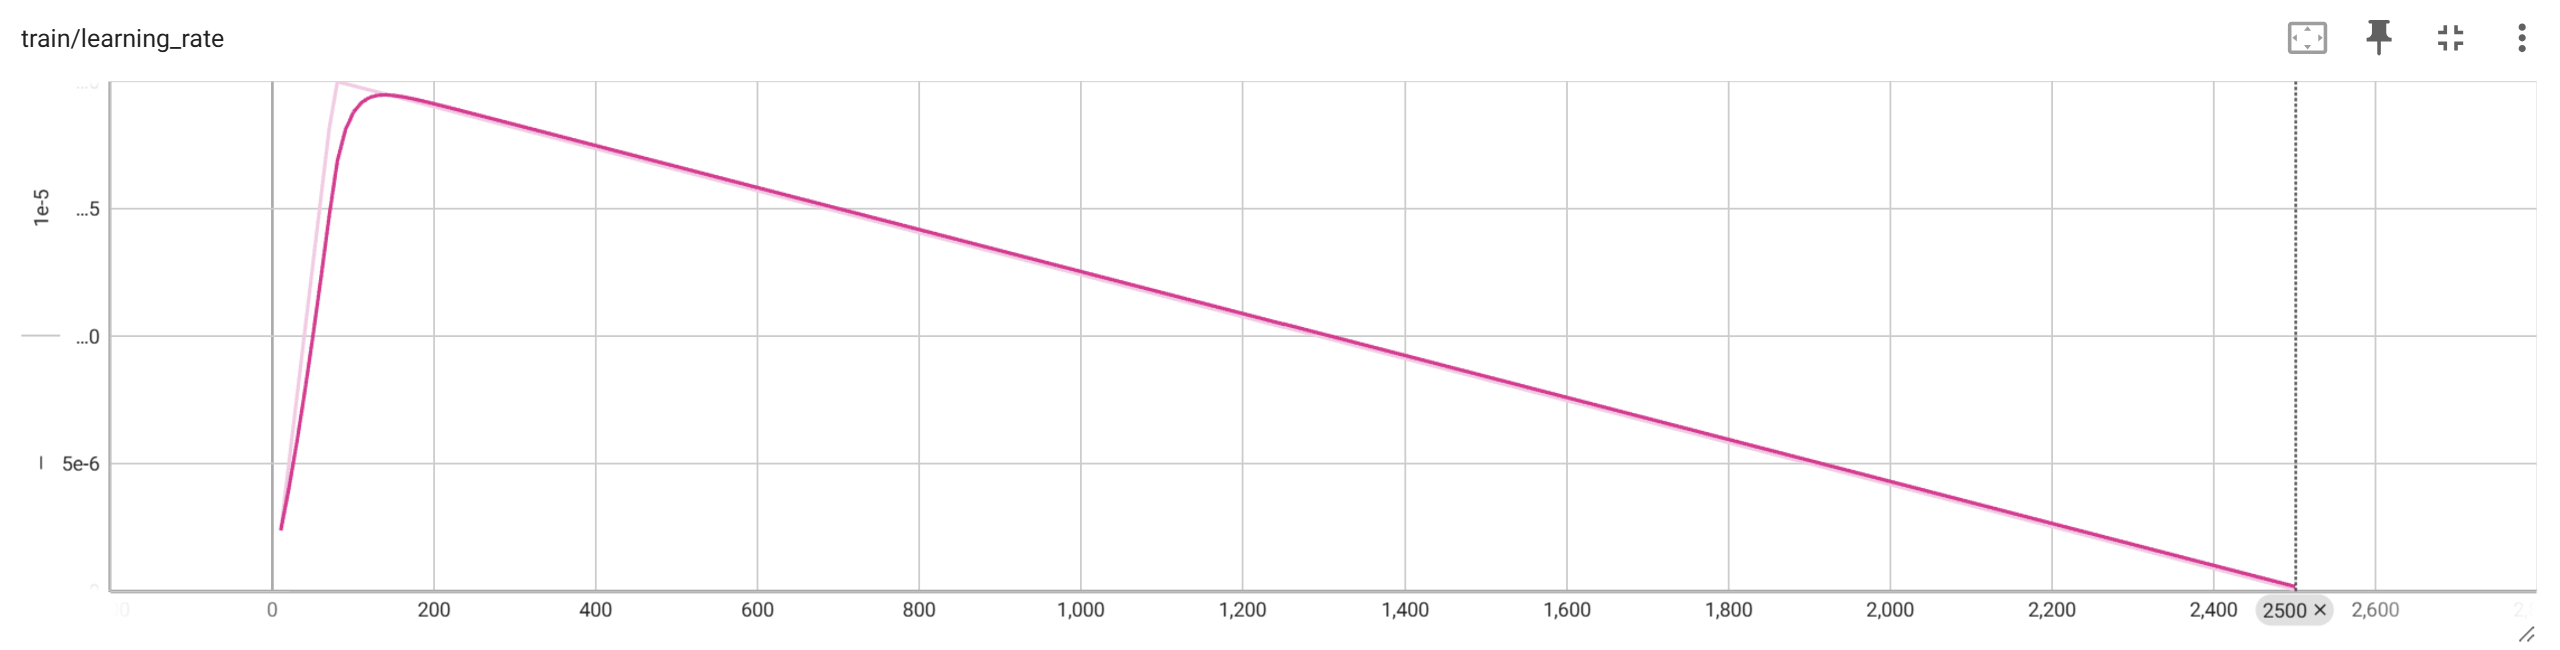
\includegraphics[width=\linewidth]{img/sctod_train_learning_rate.png}
        \caption{Learning rate}
    \end{subfigure}
    \begin{subfigure}[b]{0.49\linewidth}
        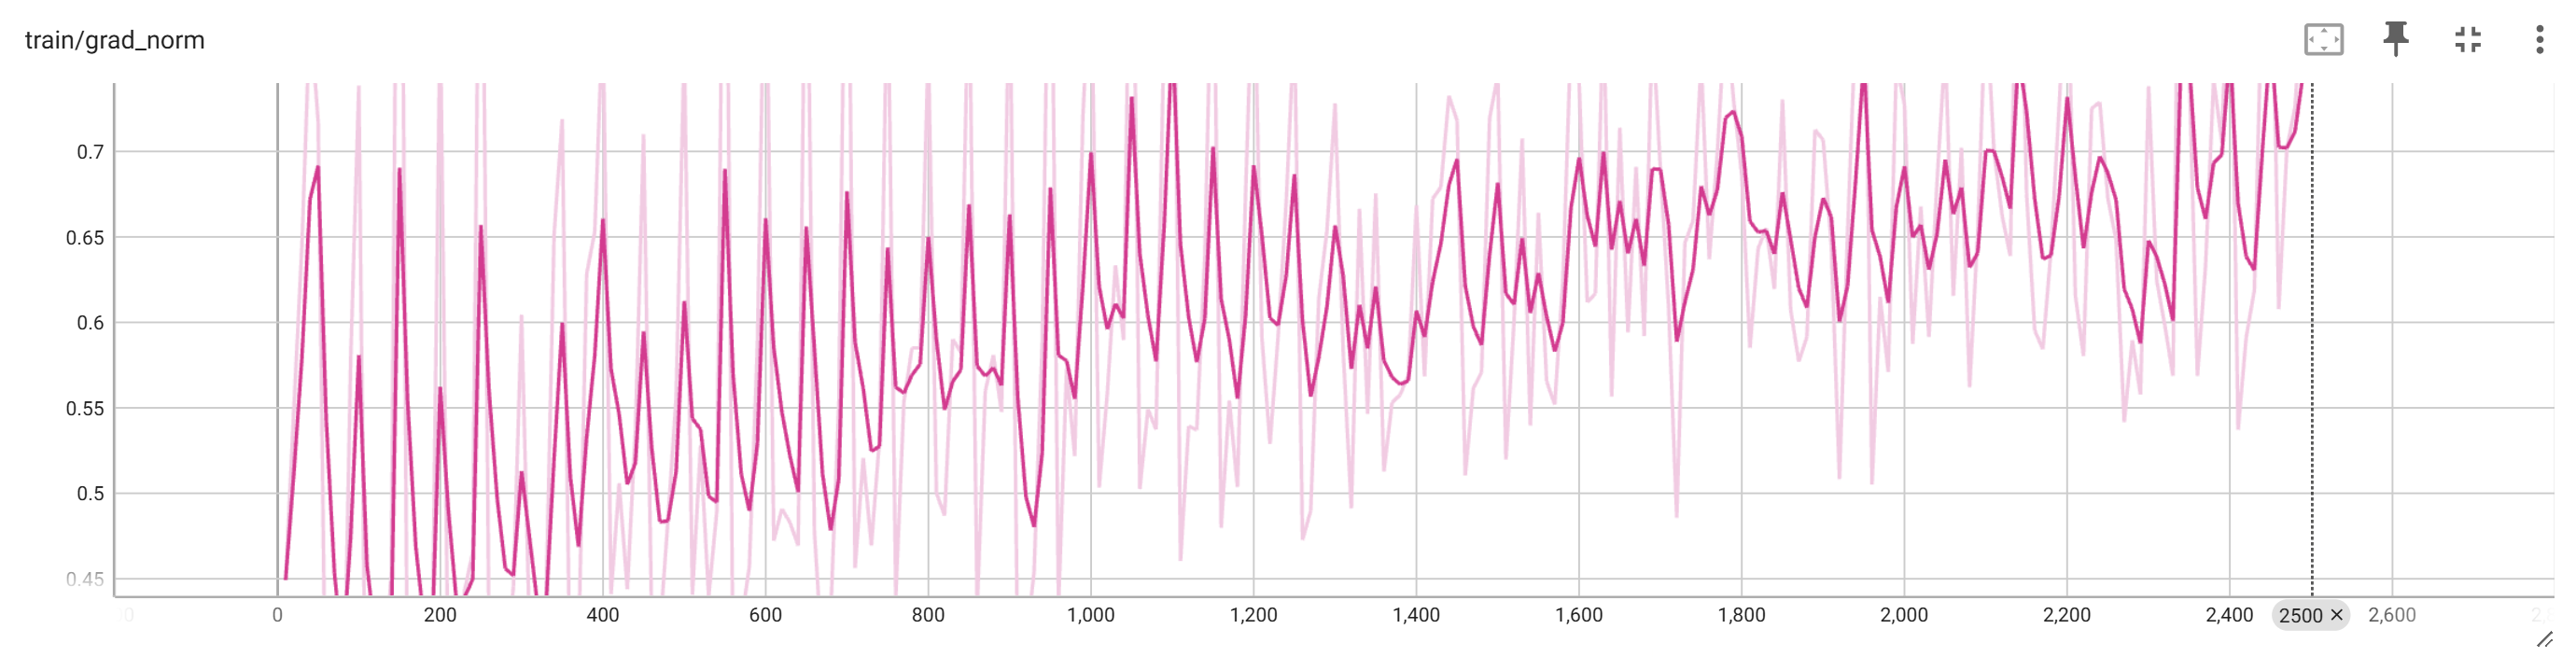
\includegraphics[width=\linewidth]{img/sctod_train_grad_norm.png}
        \caption{Grad norm}
    \end{subfigure}
    \caption{SCoTD dynamics: short warmup then linear LR decay; grad norms in a tight 0.45--0.75 band with slight late drift upward.}
    \label{fig:sctod-dynamics}
\end{figure}

Observations:
\begin{itemize}
    \item Stable optimization: absence of large spikes (Figure \ref{fig:sctod-dynamics}b) due to longer sequences distributing updates.
    \item Continued eval improvement: eval loss still falling past best accuracy checkpoint (Figure \ref{fig:sctod-losses}b) implying accuracy saturation before token-level optimum.
    \item Low variance: constrained grad norm range suggests consistent convergence; rationale diversity did not destabilize training.
\end{itemize}

\subsection{Comparison}
\begin{itemize}
    \item Label-only: faster early loss reduction (Figure \ref{fig:labelonly-losses}a) but earlier generalization peak and overfitting (Figure \ref{fig:labelonly-losses}b).
    \item SCoTD: sustained eval loss improvement (Figure \ref{fig:sctod-losses}b); accuracy plateau likely reflects reasoning ceiling rather than overfitting.
    \item Gradient behavior: high initial label-only norms (Figure \ref{fig:labelonly-dynamics}b) vs. SCoTD’s moderate steady norms (Figure \ref{fig:sctod-dynamics}b) indicate incremental adaptation with longer rationales.
\end{itemize}

\section{Output length and latency distributions}
\begin{figure}[!h]
    \centering
    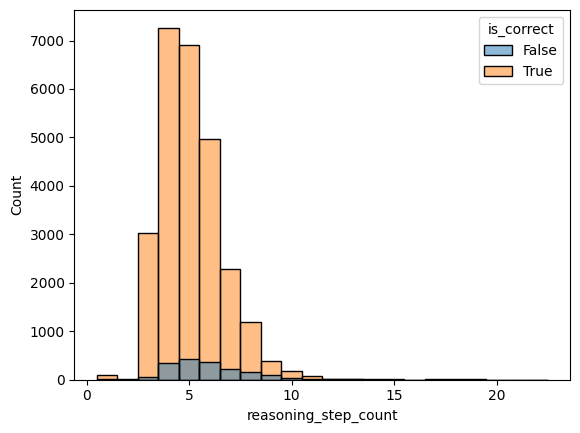
\includegraphics[width=0.48\linewidth]{img/reasoning_step_count_histogram.png}
    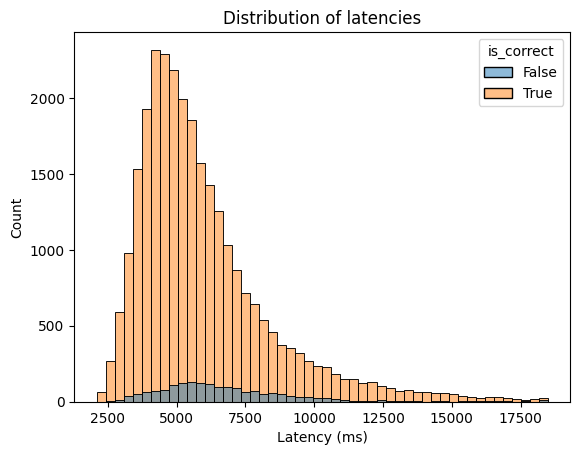
\includegraphics[width=0.48\linewidth]{img/latencies_histogram.png}
    \caption{Left: reasoning step count (mode 5, most in [4,7], rare long tails >12). Right: latency distribution (median \~5.4s, long right tail to >18s).}
    \label{fig:steps-latency}
\end{figure}

\begin{figure}[!h]
    \centering
    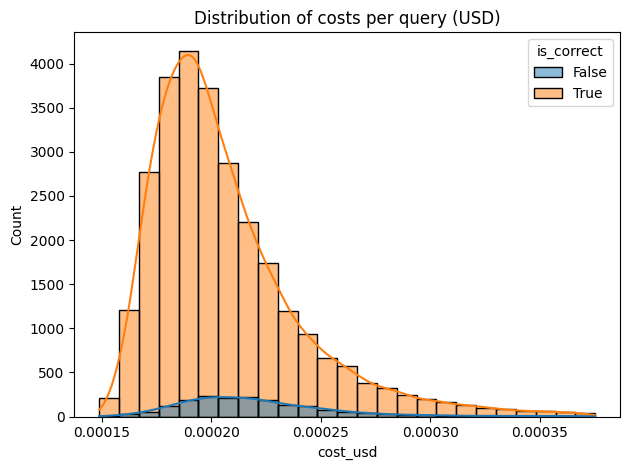
\includegraphics[width=0.295\linewidth]{img/cost_per_query_histogram.png}
    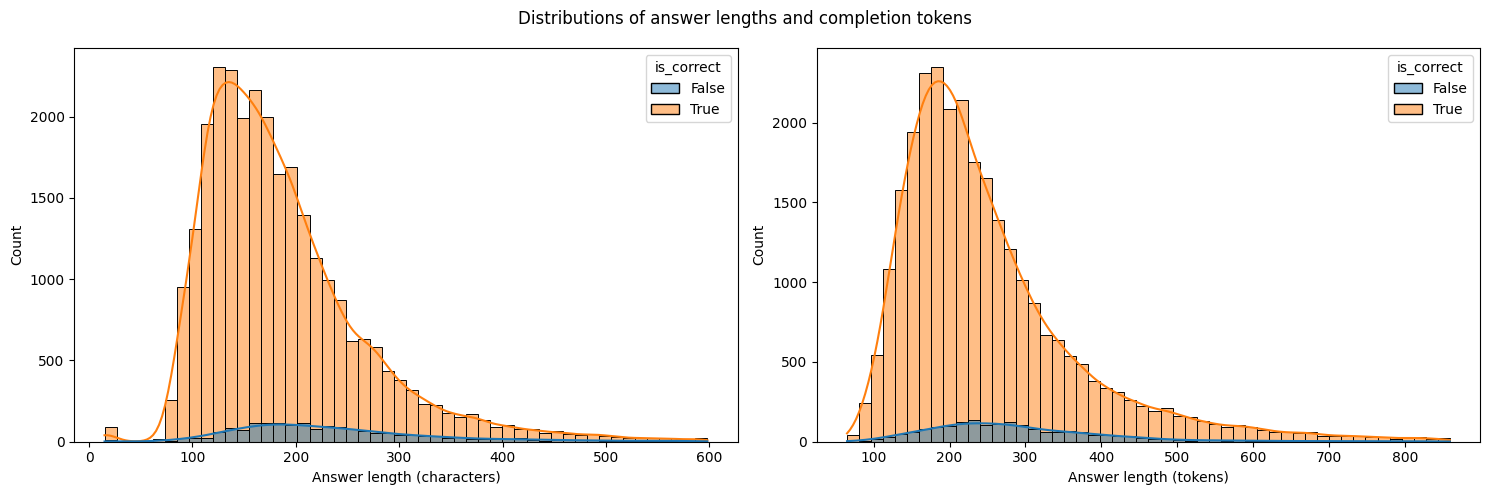
\includegraphics[width=0.685\linewidth]{img/answer_lengths_and_completion_token_histograms.png}
    \caption{Left: cost per query (right-skew, peak near \$0.00019--0.00021). Right: answer length distributions (characters and tokens; token mode \~180, tail >800).}
    \label{fig:cost-length}
\end{figure}

Quantitative summaries:
\begin{itemize}
    \item Step count: 90\% within 4--7 steps; incorrect samples slightly over-represented at 4--5 steps (shorter reasoning).
    \item Latency: interquartile band concentrated between \~4.3s and \~7.1s; heavy tail aligns with longest completions.
    \item Cost: distribution approximates log-normal; long tail beyond \$0.00030 mainly verbose rationales.
    \item Length: character median \~150; token median 225 (matches earlier quantiles); incorrect answers mildly skew shorter (information insufficiency).
\end{itemize}

\section{Dataset filtering outcomes}
\subsection{Raw and cleaned sizes}
\begin{itemize}
    \item Raw generated samples: 30{,}000 (1{,}000 train questions $\times$ 30 teacher generations).
    \item Teacher overall numeric correctness (raw): 93.75\% (28{,}125 correct).
    \item Cleaned samples retained: 24{,}952 (100\% correct after filtering).
\end{itemize}

\subsection{Removal breakdown (approximate)}
\begin{itemize}
    \item Incorrect answers removed: 1{,}875.
    \item Length outliers (>\,99th percentile total tokens; threshold $\approx$1{,}392): $\sim$300 (at most 1\%).
    \item Exact duplicate rationales removed: $\sim$2{,}873 (difference after accounting for outliers). 
\end{itemize}
Note: Duplicate vs outlier counts are approximate; precise tallies depend on overlapping removal cases.

\subsection{Effect}
Filtering ensures zero label noise and improved rationale diversity while capping worst-case sequence length for memory stability.

\section{Cost analysis}
\subsection{Aggregate}
\begin{itemize}
    \item Total teacher generation cost: \$6.33240.
    \item Average cost per raw query: \$0.00021 (median \$0.00020; std \$0.000062).
    \item Cost per retained cleaned sample: \$6.33240 / 24{,}952 $\approx$ \$0.000254.
\end{itemize}

\subsection{Distribution}
Histogram shows a right-skew with a long tail up to $\sim$\$0.00037 (Figure: cost per query). Tail samples correspond to longer completions (higher completion token counts). Tight clustering around \$0.00020 indicates stable prompt length and moderate variance in rationale length.
